\documentclass[11pt,letterpaper]{article}
\usepackage[margin=1.0in]{geometry}
\usepackage[utf8]{inputenc}
\usepackage{cite}
\usepackage{amsmath}
\usepackage{amsfonts}
\usepackage{amssymb}
\usepackage{makeidx}
\usepackage{graphicx}
\usepackage{hyperref}
\setlength\parindent{0pt}

\author{STUDENT NAME}
\title{Lab6: Ordinary Least Squares Fitting}

\begin{document}

\maketitle
 
\section{Objective}

The objective of this lab is to introduce the concept of Ordinary Least Squares fitting, and to learn how to program this algorithm in MatLab. En passé the student will learn general methods of matrix manipulation using MatLab.

\section{Introduction}

One of the most common forms of data analysis is to discover underlying themes in data. Often we use ‘best fit’ models where we assume that the mechanism that connects an input to an output can be described by a simple mathematical relationship (such as the polynomial) and we hope that the remainder (residuals) are random noise. A good example is a flow rate versus a pressure, where we make the assumption that Bernoulli's law holds, and therefore there should be a quadratic relationship between pressure and flowrate. The aim is to explain most of the data using the fewest number of terms (this is called a parsimonious model). The general polynomial model we are going to fit on the data can be written as follows:

\begin{equation} \label{Eqn:OLS1}
y = \theta_0 + \theta_1 x + \theta_2 x^2 + e
\end{equation}

where $e$ is an error term. In matrix form:

\newenvironment{spmatrix}[1]
 {\def\mysubscript{#1}\mathop\bgroup\begin{pmatrix}}
 {\end{pmatrix}\egroup_{\textstyle\mathstrut\mysubscript}}
 
\begin{equation}\label{Eqn:OLS2}
\begin{pmatrix}
y_1 \\
\vdots \\
y_n \\
\end{pmatrix}
=
\begin{pmatrix}
1 & x_1    & x_1^2\\
1 & \vdots &\vdots \\
1 & \vdots & \vdots\\
1 & x_n    & x_n^2
\end{pmatrix}
\begin{pmatrix}
\theta_0 \\
\theta_1 \\
\theta_2 \\
\end{pmatrix}
+
\begin{pmatrix}
e_1 \\
\vdots \\
e_n \\
\end{pmatrix}
\end{equation}

or

\begin{equation} \label{Eqn:OLS3}
\bar{y} = A \bar{\theta} + \bar{e}
\end{equation}

To give us the best fitting polynomial, we minimize the square of the error which gives us an Ordinary Least Squares (OLS) estimator and obtain the optimal parameter vector as follows:

\begin{equation} \label{Eqn:OLS4}
\min(e^T e) = min\left[ \left( \bar{y} - A \bar{\theta} \right)^T \left( \bar{y} - A \bar{\theta} \right)  \right] 
\end{equation}

The result is:

\begin{equation} \label{Eqn:OLS5}
\hat{\bar{\theta}} = \left(A^TA \right)^{-1} A^T y  
\end{equation}

The \href{http://en.wikipedia.org/wiki/Coefficient_of_determination}{coefficient of determination} $R^2$ indicates how good the fit is. For this we need two factors, 1) the sum of squared residuals (SSR), which is fact the sum of the squared differences between the data and the model (this is our $S = e^2 = \sum_{i}^{} e_i^2  = \sum_{i}^{} \left( y_i - f(x,\theta) \right) ^2$) and 2) the total sum of squares of the dataset as follows: $SST = \sum_{i}^{} \left( y_i - \bar{y} \right) ^2$, where $\bar y$ is the mean of $y$. The coefficient of determination is now:

\begin{equation} \label{Eqn:OLS15}
R^2 = 1 -  \dfrac{SSR}{SST}
\end{equation}

This formula shows you how you can compute the coefficients based on the regressor matrix $A$ and the data vector $y$, which contains the measurements.

\section{Procedures}

If you are not familiar (or somewhat rusty) in MatLab, do the Questions section first. Given is data vector x,y as follows (and shown in Figure \ref{fig:Lab6_OLS_Data}):

\begin{figure}
\centering
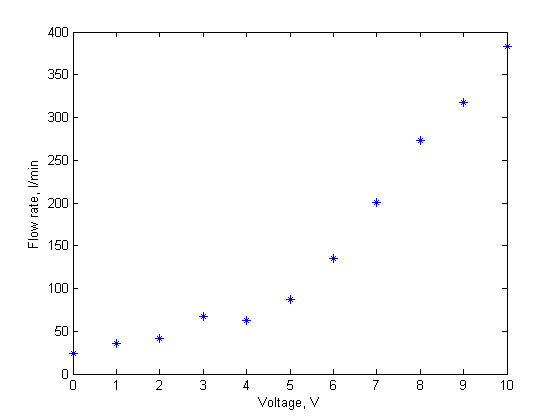
\includegraphics[width=0.8\linewidth]{Lab6_OLS_Data}
\caption{These data represent the relationship between an electric input (x-axis, Volt) and a flow rate output (y-axis, l/min).}
\label{fig:Lab6_OLS_Data}
\end{figure}

\begin{equation}\label{Eqn:OLS6}
x = 
\begin{pmatrix}
0 \\
1 \\
2 \\
3 \\
4 \\
5 \\
6 \\
7 \\
8 \\
9 \\
10\\
\end{pmatrix}
\\
y=
\begin{pmatrix}
24 \\
36 \\
42 \\
67 \\
62 \\
87 \\
135 \\
201 \\
273 \\
318 \\
383\\
\end{pmatrix}
\end{equation}

\begin{figure}
\centering
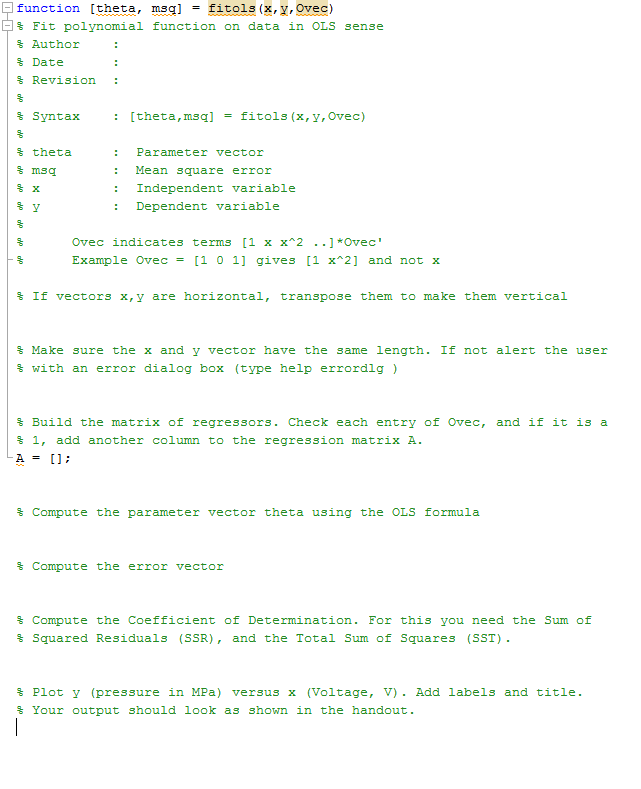
\includegraphics[width=1\linewidth]{fitols_template}
\caption{Template for the fitols function, download this file in plain text format \href{http://abe-research.illinois.edu/Faculty/grift/ABE425_2015/Labs/fitolsTemplate.txt}{here}, cut and past into MatLab's editor. You can also download the data \href{http://abe-research.illinois.edu/Faculty/grift/ABE425_2015/Labs/OLS_Data.txt}{here}. If all terms are in the model (Ovec = [1 1 1]) the output should look like Figure \ref{fig:Lab6_OLS_DataFitted}}
\label{fig:fitols_template}
\end{figure}

\begin{figure}
\centering
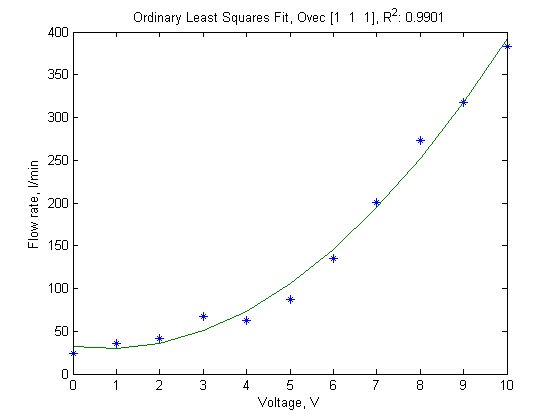
\includegraphics[width=0.8\linewidth]{Lab6_OLS_DataFitted}
\caption{These data represent the relationship between an electric input (x-axis, Volt) and a flow rate output (y-axis, l/min). The fit parameters are shown in the title.}
\label{fig:Lab6_OLS_DataFitted}
\end{figure}

\begin{enumerate}

\item In MatLab, build the regressor matrix

\begin{equation}\label{Eqn:OLS7}
A =
\begin{pmatrix}
1 & x_1    & x_1^2\\
1 & \vdots &\vdots \\
1 & \vdots & \vdots\\
1 & x_n    & x_n^2
\end{pmatrix}
\end{equation}

\item Compute the coefficient vector $\hat{\bar{\theta}} = \left(A^TA \right)^{-1} A^T y$ in a single MatLab statement.
\item Plot the original data.
\item Plot the model as $\bar{y} = A \bar{\theta} $ in the same figure. Type "help hold" for this.
\item Plot the error in a separate figure.
\item Compute the square of the error $e^T e$.
\item Build a generic routine where the user can select which terms are going to be in the model and which are not. Think about how to set up your regressor matrix related to the Order Vector Ovec as described in the template Figure \ref{fig:fitols_template}.
\end{enumerate}

\section{Questions}

Q1:	What is the dimension of a product of an n*m matrix times an m*1 vector? \\
A1:\\


Q2: What is the dimension of a product of a 1*m vector times an m*1 vector? What is the name of a matrix with this dimension? \\
A2:\\

Q3:	What is the dimension of a product of an m*1 vector times a 1*m vector \\
A3:\\


Q4: Sometimes instead of a vector product, we simply want to multiply all the entries of the vector with each other, resulting in a vector of the same dimension as the original vectors. How does one do this in MatLab? \\
A4:\\

Q5: Given are the following matrices and vector.

\begin{equation}\label{Eqn:OLS8}
a =
\begin{pmatrix}
4 & 9    & 2\\
3 & 5 & 7\\
8 & 1  & 6\\
\end{pmatrix}
b=
\begin{pmatrix}
7 & 9    & 3\\
3 & 6 & 2\\
5 & 1  & 4\\
\end{pmatrix}
c=
\begin{pmatrix}
2 \\
3 \\
-1 \\
\end{pmatrix}
\end{equation}

Compute:\\

\begin{align}
a+b & = \\
a*c & =\\
a^T & =\\
a^{-1} & =\\
c^T*c & =\\
c*c^T & =\\
c.*c & =\\
(a^T a )^{-1} a^T c &=\\
\end{align}

A5:\\

\end{document}